\documentclass{article}

\usepackage{mathtools,amsfonts}
\usepackage{enumerate}
\usepackage{fullpage}
\usepackage{fancyvrb}


\begin{document}
\thispagestyle{empty}

\begin{center}
  \textbf{\Large Intermediate Test 1}
  % LEVEL is Senior, Intermediate or Beginner
  % NUMBER is the test number: 1, 2, etc.
  \\ \vspace{1em}
  \textbf{\large January Camp 2021}
  \\ \vspace{1em}
  \textbf{\large Time: $2\frac{1}{2}$ hours}
\end{center}

\vspace{24pt}

\begin{enumerate}[1.]

\item You are given the following shape: % South Africa, Tim's Assorted Combinatorics Questions 2020, Q2
	\begin{center}
	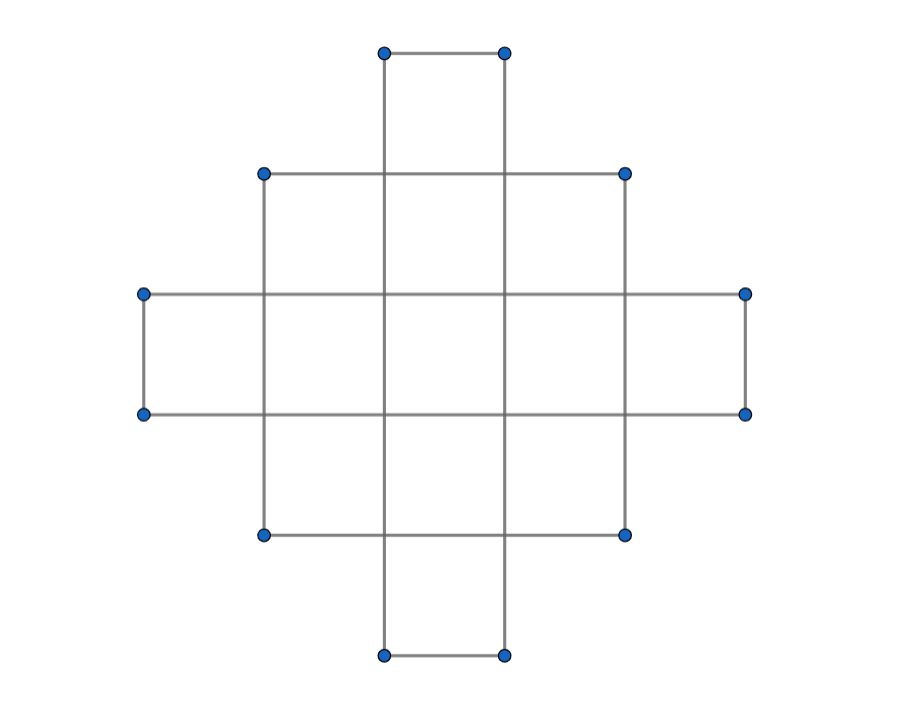
\includegraphics[scale=0.3]{Capture.png}	
	\end{center}
You need to tile this with L-shapes made of 3 blocks. Which single blocks could you shade out of the original diagram to make this possible?


\item % Ukraine 2016-2017, Third Round 2017, First Tour, 4.1
Let $ABCD$ be a trapezoid with $AD \parallel BC$. The angle bisector of $\angle DAB$ intersects the angle bisectors of $\angle ABC$ and $\angle CDA$ at points $P$ and $S$ respectively, and the angle bisector of $\angle BCD$ intersects the angle bisectors of $\angle ABC$ and $\angle CDA$ at points $Q$ and $R$ respectively. Furthermore, $PS \parallel RQ$. Prove that $AB = CD$.


\item % Moldova, 61st Maths Olympiad (2017), 7.1 modified
Find all natural numbers $x$, $y$ and $z$ satisfying 
$$x + \frac{1}{y + \frac{1}{z}} = \frac{850862}{421}$$


\item % Ukraine 2018-2019, 3rd round, second tour, 9th Grade, Q1
Find all possible real numbers $k$ such that the values of $x$ satisfying
$$k(2 - k)x^2 - (k + 4)x + 6 = 0$$
are positive integers.


\item % Ireland, 2017, Powerful Sequences, Q2
Let $O$ be the circumcentre of $\triangle ABC$. Let $X$, $Y$ and $Z$ be the reflections of $O$ over $AB$, $BC$ and $CA$ respectively. Prove that $\triangle XYZ$ is congruent to $\triangle ABC$ and the corresponding sides are parallel.



\end{enumerate}


\vfill
% ASCII art
\centering
\begin{BVerbatim}
 >(·)__ <(·)__ =(·)__
  (___/  (___/  (___/ 
\end{BVerbatim}

\end{document}
